\section{Controller Analysis}\label{ssec:ControllerVerification}
A further analysis can be done to the controller, both continuous and discrete, and also to the real response of the system once it is implemented.

The first step is to simulate both the continuous and discrete controller with the model of the system and analyse the behavior of the whole closed loop system.

This is done not only to see the behavior of the designed controller but also to verify that the discretized controller matches the original continuous one. 

With a constant reference of 0 rad and a disturbance in the form of a torque applied to the frame of \si{0,55 Nm}, the responses are the ones shown in \figref{discreteVsContinuousOutputController} and \figref{discreteVsContinuousSimulation}.
%
\begin{minipage}{0.45\linewidth}
	\begin{figure}[H]
      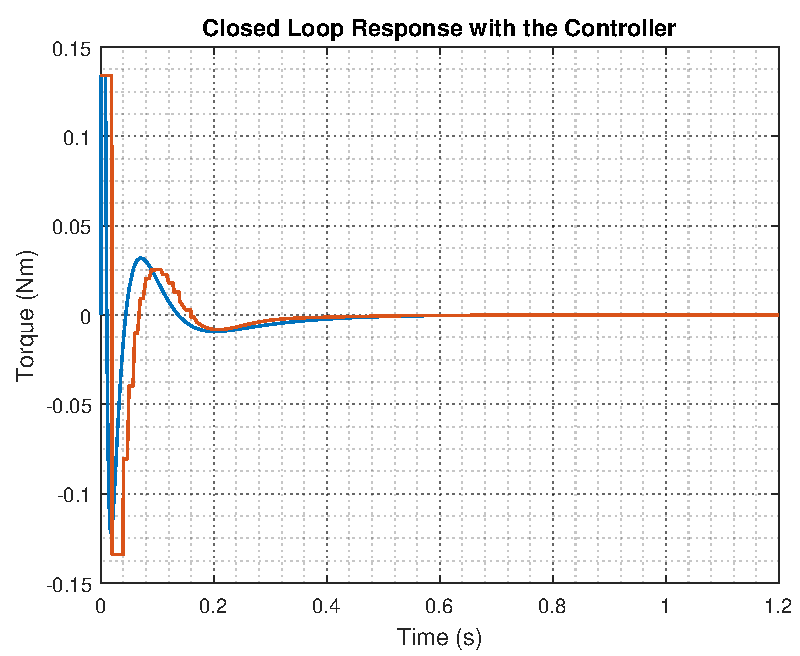
\includegraphics[scale=.53]{figures/torqueComp}
      \captionsetup{justification=centering}
      \captionof{figure}{Controller's output (torque) response in the control loop with the continuous (blue) and discrete (red) controllers}
      \label{discreteVsContinuousOutputController}
    \end{figure}\vspace{-5mm}
\end{minipage}
\hspace{0.03\linewidth}
\begin{minipage}{0.45\linewidth}
    \begin{figure}[H]\vspace{-4mm}
      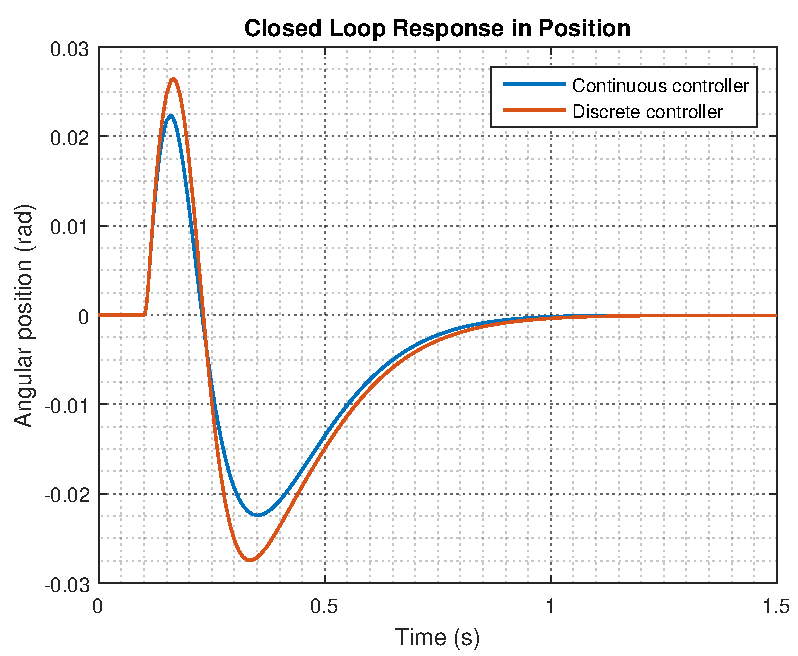
\includegraphics[scale=.53]{figures/positionComp}
      \captionsetup{justification=centering}
      \captionof{figure}{Closed loop response of the continuous (blue) and discrete (red) controllers}
      \label{discreteVsContinuousSimulation}
    \end{figure}\vspace{-5mm}
\end{minipage}

Both controllers seem to have a good behavior and both reach the desired final position. However it is important to also look at the velocity of the wheel, since it has been assumed to be 0 in the equilibrium position.
%
\begin{figure}[H]\vspace{-4mm}
	\centering
	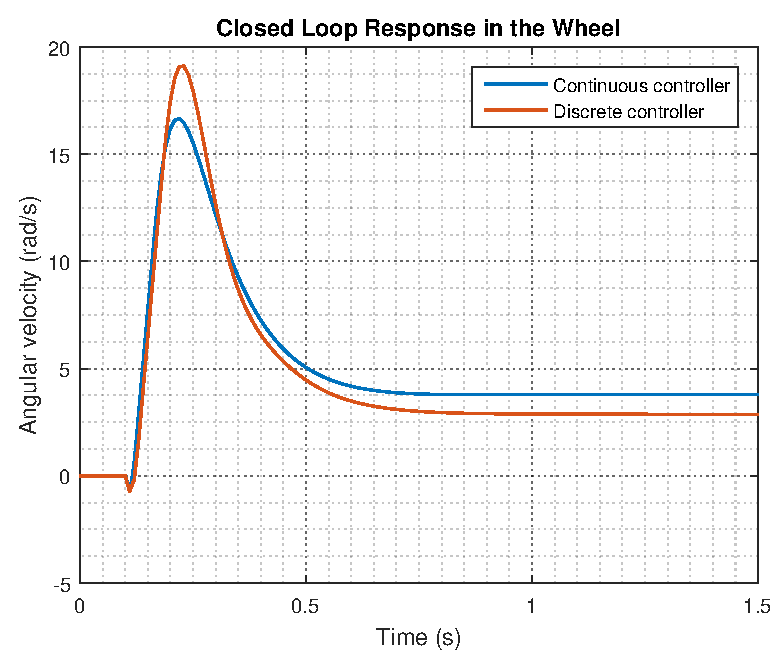
\includegraphics[scale=.53]{figures/wheelComp}
	\captionof{figure}{Angular velocity of the wheel}
   \label{fig:discreteVsContinuousWheel}
\end{figure}\vspace{-5mm}

In both cases the velocity is different from 0 in steady state. It should not be any problem since a constant velocity does not produce any torque 
to the system, but since there is friction in the wheel it will start to slow down, producing an acceleration on the system. This will make the Cubli to slightly move from equilibrium position and the controller will try to apply some torque to the system to balance it. The problem is that if the motor was already very closed to its maximum speed it will not be able to accelerate more and produce the torque needed, making the frame to fall.

The conclusion is that the controller is not able to assure zero velocity in equilibrium. This means that another kind of controller, which also takes care of the velocity of the wheel, may result in a better behavior.

One way could be using a cascade controller to control both the velocity of the wheel and the position of the frame. 

\fxnote{Include block diagram for cascade}

The problem of this solution in the case of the Cubli is that both are coupled together, which means that it is not possible to split the plant in a way that there is no feedback between them. \fxnote{reference revolutionary paper}

Another way is to use an state-space approach since now the system will have two outputs to control, and it can also take care of coupled systems. This controller solution is further detailed in \chapref{chap:stateSpaceController}.
